%%%%%%%%%%%%%%%%%%%%%%%%%%%%%%%%%%%%%%%%%
% University/School Laboratory Report
% LaTeX Template
% Version 3.1 (25/3/14)
%
% This template has been downloaded from:
% http://www.LaTeXTemplates.com
%
% Original author:
% Linux and Unix Users Group at Virginia Tech Wiki 
% (https://vtluug.org/wiki/Example_LaTeX_chem_lab_report)
%
% License:
% CC BY-NC-SA 3.0 (http://creativecommons.org/licenses/by-nc-sa/3.0/)
%
%%%%%%%%%%%%%%%%%%%%%%%%%%%%%%%%%%%%%%%%%

%----------------------------------------------------------------------------------------
%	PACKAGES AND DOCUMENT CONFIGURATIONS
%----------------------------------------------------------------------------------------

\documentclass{article}

%\usepackage[version=3]{mhchem} % Package for chemical equation typesetting
%\usepackage{siunitx} % Provides the \SI{}{} and \si{} command for typesetting SI units
\usepackage{graphicx} % Required for the inclusion of images
\usepackage{natbib} % Required to change bibliography style to APA
\usepackage{amsmath} % Required for some math elements 
\usepackage{listings}
\usepackage[a4paper, total={6in, 8in}]{geometry}
\lstset{basicstyle=\small\ttfamily, breaklines=true}
\setlength\parindent{2pt} % Removes all indentation from paragraphs
\linespread{1.8}
%\renewcommand{\labelenumi}{\alph{enumi}.} % Make numbering in the enumerate environment by letter rather than number (e.g. section 6)

%\usepackage{times} % Uncomment to use the Times New Roman font

%----------------------------------------------------------------------------------------
%	DOCUMENT INFORMATION
%----------------------------------------------------------------------------------------

\title{Laboratory on Linux Kernel Haking \\ OS - Operating System} % Title

\author{Simone \textsc{Rossi}} % Author name

\date{\today} % Date for the report

\begin{document}

\maketitle % Insert the title, author and date

\begin{center}
\begin{tabular}{l r}
Date Performed: & \today \\ % Date the experiment was performed
Partners: & Simone Rossi \\ % Partner names
%& Mary Smith \\
%Instructor: & Professor Smith % Instructor/supervisor
\end{tabular}
\end{center}

% If you wish to include an abstract, uncomment the lines below
% \begin{abstract}
% Abstract text
% \end{abstract}

%----------------------------------------------------------------------------------------
%	SECTION 1
%----------------------------------------------------------------------------------------

\section{Compiling the Linux kernel}
To analyze thet version of the kernel currently under execution, the command to be typed is 
\texttt{uname -vr}\footnote{The command returns both the kernel version and release}.\\

From the source code of \texttt{linux-2.4}, I tried to remove the support for the Ext3 
filesystem. The new kernel has been compiled (computing all the dependencies and compiling
all the sources) and mounted using \texttt{lilo}.\\

Of course now, without the support for this version of filesystem, the kernel could not correctly 
load and mount the root filesystem; as conseguence, it entered in the kernel panic state (with error
19) with no possibilities to be recovered.\\

\begin{figure}
\centering
  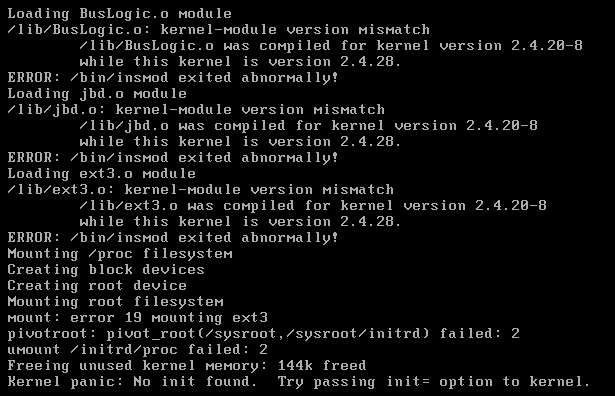
\includegraphics[width=0.8\textwidth]{./kernel_panic.png}
\end{figure}


\section{Adding new system calls to Linux}
The man page of Linux describes the system call as a fundamental interface between an application and
the Linux kernel itself. [\dots] Usually they are not invoked directly but rather via wrapper functions.\\

The system calls deal with low aspects of the operating systems, while providing high-level Application
Programming Interface (API), allowing the user to work trasparantelly without dealing with hardware - software integretion. 
Let's assume the user application calls a library function which actually during its execution makes a
system call to the kernel. The name of the system call is used as offset in a system call table and 
an interrupt is raised.\\ 

\begin{figure}[h!]
\centering
  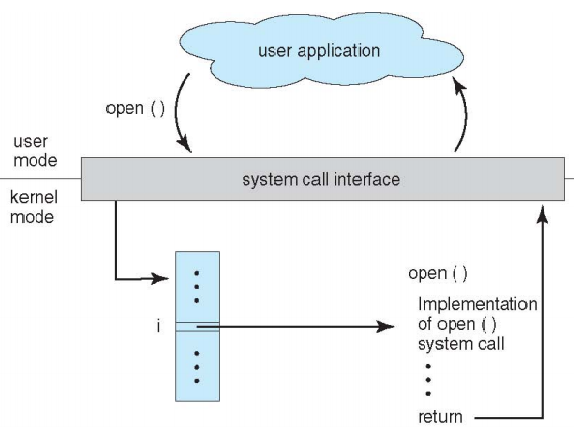
\includegraphics[width=0.6\textwidth]{./syscall.png}
\end{figure}

\newpage
As explained in the document, to add new system calls to the kernel, two files should be modified.\\
\begin{minipage}{0.4\textwidth}
  \texttt{include/asm-i386/unistd.h} contains the system call numbers for the system call table
  and seven different template prototype for the function (with different numbers of parameters).
\end{minipage}
\begin{minipage}{0.65\textwidth}
  \centering
  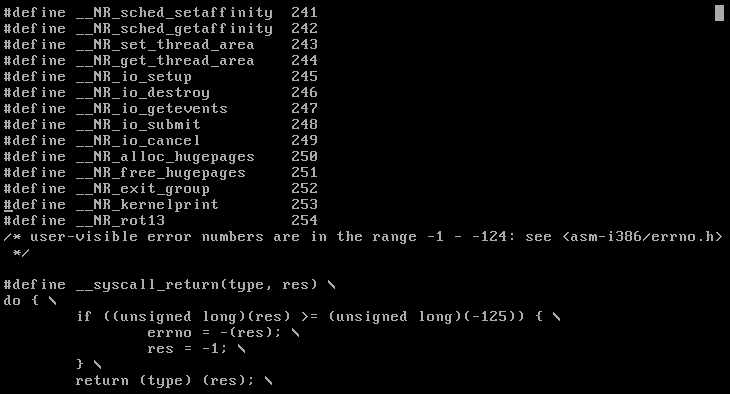
\includegraphics[width=.8\textwidth]{./unistd.png}
\end{minipage}
\begin{minipage}{0.4\textwidth}
\texttt{arch/i386/kernel/entry.S} contains the system call low level handling routines and 
       the link between a system call and a entry of the systel call table.
\end{minipage}
\begin{minipage}{0.65\textwidth}
  \centering
  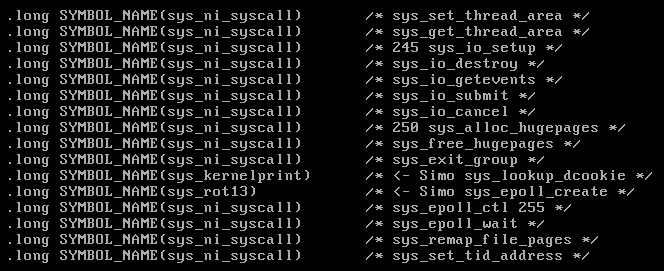
\includegraphics[width=.8\textwidth]{./entrys.png}
\end{minipage}
\\


Up to now, I have only the defined the entry point for my future kernel calls but actually no function has been 
written yet. For this point, writing a system call has not big differences with respect to normal library functions:
prototypes will be declared in a dedicated \texttt{.h} file and the source in a \texttt{.c} file. Anyway, the execution
of a system call is radically different.\\

The paths in which these files will be saved should not be constrained; anyway, following the nominal convention, the header
has been saved in \texttt{include/linux} (since is hardware independent), while the source simply in \texttt{kernel/}.\\

In the following pictures, both header and source will be present.

\begin{figure}[h!]
  \centering
  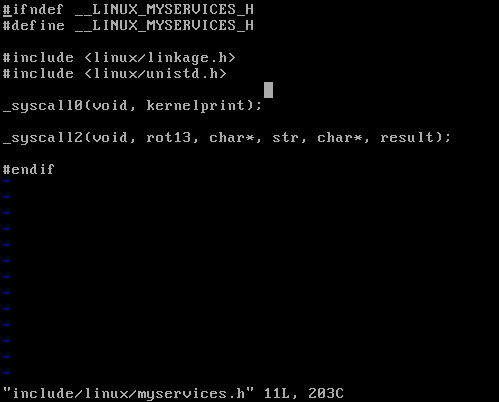
\includegraphics[width=0.9\textwidth]{./services_h.png}
  \caption{\texttt{myservices.h} content}
\end{figure}


\begin{figure}[h!]
  \centering
  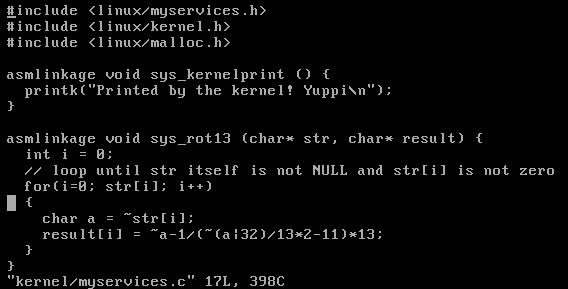
\includegraphics[width=0.9\textwidth]{./services_c.png}
  \caption{\texttt{myservices.c} content}
\end{figure}

\texttt{kernelprint()} is the same function provided in the document and simply print (using \texttt{printk}) a message on the terminal. 
It has been defined as a system call that takes no parameters and returns to void. \\

On the other hand, \texttt{rot13(\dots)} is more complex.
To avoid problems related to memory allocation and data copy between kernel space and user space (which eventually may lead to a Segmentation Fault),
the function has been defined with two parameters (the pointer to the original string and the pointer to the modified one) and returns to void.
For the function, the return string has supposed to be already allocated and pointing to a valid memory address.
\\

The functions are now defined and written; to make them available as system calls, the kernel should be recompiled (note that the Makefile should
be updated with the new required object).\\

Let's look at the definition of a function; one small detail identify the function to behave as a system call: the flag \texttt{asmlinkage}.
This access identifier tells to the GCC compiler to look on the CPU stack for the function parameters, instead of registers.
As aforementioned, system calls are services that user space can call to request the kernel to perform something for them (and therefore execute in kernel space). 
These functions will not behave like normal functions, where parameters are typically passed by writing to the program stack, but instead they are written to registers.
While still in userspace, calling a syscall requires writing certain values to certain registers is translated.
The system call number will always be written in \texttt{eax}, while the the rest of the parameters will go into \texttt{ebx}, \texttt{ecx}, etc. 
The CPU is interrupt with a software \texttt{int} and the switches to kernel mode to then execute \texttt{system\_call()}.
So, since all the information about the parameters passed all the way from userland to this point is nicely stored in the stack, the compiler must be instructed about this.
\let\thefootnote\relax\footnote{https://www.quora.com/Linux-Kernel-What-does-asmlinkage-mean-in-the-definition-of-system-calls}

After the recompiling operation has been completed, the system has been reboot on the new kernel and this is the result of the use of these two new system calls.

\begin{figure}
  \centering
  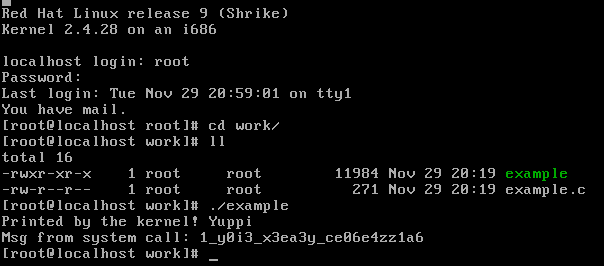
\includegraphics[width=\textwidth]{./result.png}
  \caption{Examples of system call use}
\end{figure}


\section{Optimize kernel size}
I tried different configuratios of the kernel, starting both from a full custom and tuning the default one. The smallest bootable kernel I could compile was about 600 KB (with respect of more than 850 KB with default configuration is about 30\% less). In the following pictures, the kernel size and the proof of the system calls are presented. A lot of errors appear but the system call still works.  

\begin{figure}
  \centering
  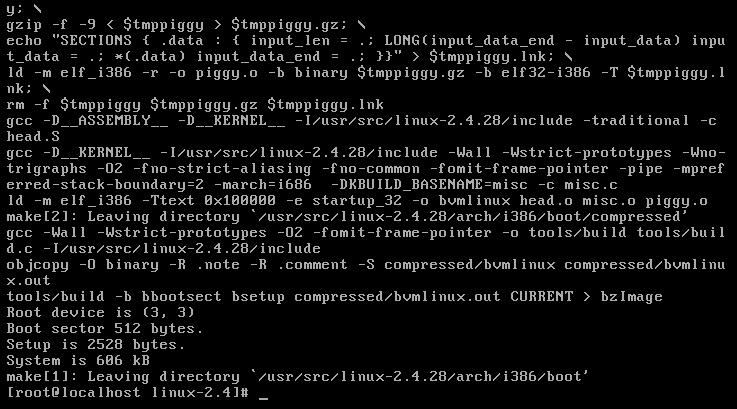
\includegraphics[width=\textwidth]{./small2.png}
\end{figure}

\begin{figure}
  \centering
  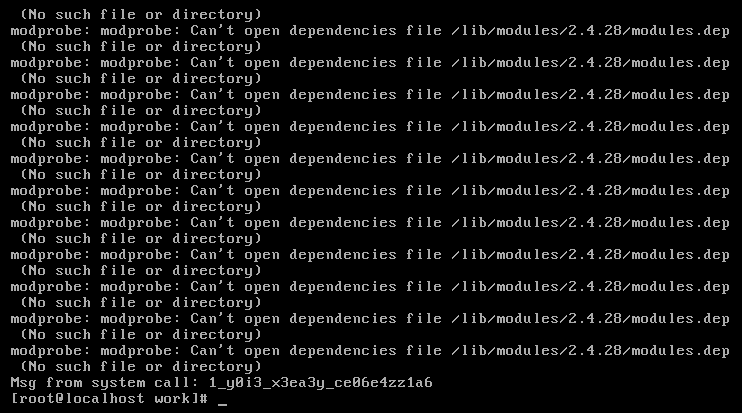
\includegraphics[width=\textwidth]{./small_example.png}
\end{figure}
\end{document}
